\documentclass[12pt, twoside, a4paper, hidelinks]{article}

    \usepackage{amsmath}
    \usepackage[utf8]{inputenc}
    \usepackage{graphicx}
    \usepackage[L7x,T1]{fontenc}
    \usepackage[utf8]{inputenc}
    \usepackage[lithuanian]{babel}
    \usepackage[left=3cm,right=1cm,top=3cm,bottom=2cm]{geometry}
    \usepackage{lipsum}  
    \usepackage{tikz}
    \usepackage{circuitikz}
    \usepackage{float}
    \usepackage{vwcol}
    \usepackage{blindtext}
    \usepackage{hyperref}
    \usepackage{enumitem}
    \usepackage[1]{pagesel}
    \setlist{leftmargin=8mm}
    \addtolength\oddsidemargin{-1cm} \addtolength\evensidemargin{1cm}
    \graphicspath{ {images/} }
    \usepackage{indentfirst}
    \usepackage{caption}
    \captionsetup[table]{labelsep=period}
    \captionsetup[figure]{labelsep=space}
    \pagestyle{empty}
    \begin{document}
    \begin{center} {\large \textbf{Abstract Title}} \end{center}
    \begin{center} First Name, Second Author \end{center}

    \begin{center} 1
        
        22
        
        email@email.com
    \end{center}

    \lipsum[2]
\begin{figure}[H]
\center
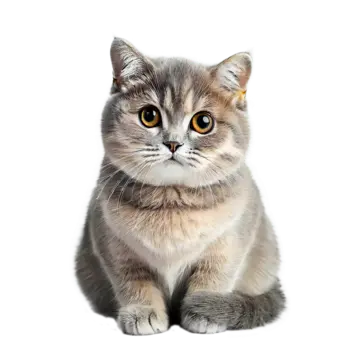
\includegraphics[height=6cm]{cat}
\caption{Katinas}
\end{figure}
\lipsum[2]
\begin{equation}
\int_a^b x^2 dx = \cfrac{x^3}{3}
\end{equation}
\lipsum[2]

    \setcounter{footnote}{1} \footnotetext{Reference}
        \setcounter{footnote}{2} \footnotetext{Book}
        
    \end{document}